%%%%%%%%%%%%%%%%%%%%%%%%%%%%%%%%%%%%%%%%%%%%%%%%%%%%%%%%%%%%%%%%%%%%%%%%%%%%%%%
%                       CARGA DE LA CLASE DE DOCUMENTO                        %
%%%%%%%%%%%%%%%%%%%%%%%%%%%%%%%%%%%%%%%%%%%%%%%%%%%%%%%%%%%%%%%%%%%%%%%%%%%%%%%

\documentclass[11pt,spanish,listoffigures,listoftables]{tfgetsinf}

%%%%%%%%%%%%%%%%%%%%%%%%%%%%%%%%%%%%%%%%%%%%%%%%%%%%%%%%%%%%%%%%%%%%%%%%%%%%%%%
%                          CODIFICACIÓN DEL FICHERO                           %
%%%%%%%%%%%%%%%%%%%%%%%%%%%%%%%%%%%%%%%%%%%%%%%%%%%%%%%%%%%%%%%%%%%%%%%%%%%%%%%

\usepackage[utf8]{inputenc} 
\usepackage{babel}
\usepackage{hyperref}
\usepackage{biblatex}
\usepackage{amsmath, amssymb}
\usepackage{graphicx}
\usepackage{booktabs}
\usepackage{listings}
\usepackage{xcolor}
\usepackage{multirow}
\usepackage{subcaption}

 

\addbibresource{bib.bib}  % Enlazar el archivo .bib
\addglobalbib{bib.bib}
\hypersetup{ colorlinks=true, linkcolor=black, urlcolor=cyan }

%%%%%%%%%%%%%%%%%%%%%%%%%%%%%%%%%%%%%%%%%%%%%%%%%%%%%%%%%%%%%%%%%%%%%%%%%%%%%%%
%                             OTROS PAQUETES                                  %
%%%%%%%%%%%%%%%%%%%%%%%%%%%%%%%%%%%%%%%%%%%%%%%%%%%%%%%%%%%%%%%%%%%%%%%%%%%%%%%

%%%%%%%%%%%%%%%%%%%%%%%%%%%%%%%%%%%%%%%%%%%%%%%%%%%%%%%%%%%%%%%%%%%%%%%%%%%%%%%
%                         DATOS DEL TRABAJO                                   %
%%%%%%%%%%%%%%%%%%%%%%%%%%%%%%%%%%%%%%%%%%%%%%%%%%%%%%%%%%%%%%%%%%%%%%%%%%%%%%%

\title{Clasificación automática de artrosis en rodillas mediante redes neuronales convolucionales}
\author{Hernández Martínez, Carlos}
\tutor{Juan Ciscar, Alfonso}
\curs{2024-2025}

%%%%%%%%%%%%%%%%%%%%%%%%%%%%%%%%%%%%%%%%%%%%%%%%%%%%%%%%%%%%%%%%%%%%%%%%%%%%%%%
%            PALABRAS CLAVE Y RESÚMENES (en tres idiomas)                     %
%%%%%%%%%%%%%%%%%%%%%%%%%%%%%%%%%%%%%%%%%%%%%%%%%%%%%%%%%%%%%%%%%%%%%%%%%%%%%%%

\keywords{Palabras clave en catalán} % catalán
         {Palabras clave en español} % español
         {Keywords in English}       % inglés

% Añade esto en el preámbulo (antes de \begin{document})
\setcounter{tocdepth}{1} % Muestra solo capítulos y secciones en el índice
\begin{document}

%%%%%%%%%%%%%%%%%%%%%%%%%%%%%%%%%%%%%%%%%%%%%%%%%%%%%%%%%%%%%%%%%%%%%%%%%%%%%%%
%                             RESÚMENES                                       %
%%%%%%%%%%%%%%%%%%%%%%%%%%%%%%%%%%%%%%%%%%%%%%%%%%%%%%%%%%%%%%%%%%%%%%%%%%%%%%%

\begin{abstract}
Aquí citamos a un datajkjkset \cite{gornale2020digital}.
Citación paper IEE \cite{10863523}, Dataset \cite{chen2018knee}
aqui citamos un paper \cite{VAATTOVAARA2025100580}
otra cita \cite{comprehensive_review}

Quitar imagenes brillantes -> \cite{efficientnet_paper}
\end{abstract}

\begin{abstract}[spanish]
(Resumen en castellano)
\end{abstract}

\begin{abstract}[english]
(Resumen en inglés)
\end{abstract}

\mainmatter

%%%%%%%%%%%%%%%%%%%%%%%%%%%%%%%%%%%%%%%%%%%%%%%%%%%%%%%%%%%%%%%%%%%%%%%%%%%%%%%
%                              CAPÍTULO 1                                     %
%                                    INTRO                                     %
%%%%%%%%%%%%%%%%%%%%%%%%%%%%%%%%%%%%%%%%%%%%%%%%%%%%%%%%%%%%%%%%%%%%%%%%%%%%%%%

\chapter{Introducción}  % ~5 páginas

\section{Motivación}     % 1.1
La artritis es una de las enfermedades musculoesqueléticas más prevalentes a nivel mundial y una de las principales causas de discapacidad en adultos mayores. Su diagnóstico y seguimiento se basa tradicionalmente en la evaluación clínica y en la interpretación de imágenes médicas, como radiografías, resonancias magnéticas y tomografías computarizadas. Sin embargo, este proceso suele depender en gran medida de la experiencia del profesional médico, lo que puede generar variabilidad en los diagnósticos y retrasos en la detección temprana de la enfermedad.

En los últimos años, los avances en inteligencia artificial, y en particular en el aprendizaje profundo, han demostrado un gran potencial para mejorar la precisión y la eficiencia en el análisis de imágenes médicas. Las redes neuronales convolucionales (CNN) han sido ampliamente utilizadas en el campo de la visión por computadora para tareas como la detección de patologías en radiografías, la segmentación de tejidos en resonancias magnéticas y la clasificación de niveles de severidad en enfermedades degenerativas.

Este Trabajo de Fin de Grado (TFG) se motiva por la necesidad de desarrollar métodos automáticos y robustos para el análisis de la artritis mediante el uso de técnicas de aprendizaje profundo. En particular, se busca explorar el uso de redes neuronales para la clasificación de imágenes médicas, utilizando bases de datos estandarizadas como \textit{Mendeley dataset} \cite{chen2018knee}. La aplicación de estos modelos podría no solo optimizar el proceso de diagnóstico, sino también contribuir al desarrollo de herramientas de soporte a la decisión clínica, facilitando una intervención más temprana y personalizada para los pacientes.

La relevancia de este estudio radica en su potencial impacto en la práctica clínica. Un sistema basado en inteligencia artificial podría reducir la carga de trabajo de los especialistas, mejorar la objetividad del diagnóstico y ofrecer segundas opiniones automáticas que complementen la evaluación médica tradicional. Además, el desarrollo de estas tecnologías en el ámbito de la artritis podría sentar un precedente para su aplicación en otras enfermedades musculoesqueléticas, ampliando el alcance del aprendizaje profundo en el campo de la salud.

Además, se plantea la posibilidad de realizar \textit{transfer learning} utilizando modelos preentrenados en artritis humana para aplicarlos en el diagnóstico de artritis en gatos. Esta adaptación podría beneficiar la práctica veterinaria, proporcionando herramientas automatizadas para la evaluación de la enfermedad en animales y mejorando la precisión en su diagnóstico.

En este contexto, el presente trabajo busca contribuir al avance del uso de inteligencia artificial en la detección y análisis de la artritis, evaluando diferentes enfoques de redes neuronales y analizando su rendimiento en la clasificación de imágenes médicas. La motivación principal es demostrar la viabilidad y efectividad de estos modelos en un problema biomédico concreto, promoviendo la integración de tecnologías emergentes en el ámbito de la salud.


\section{Objetivos}      % 1.2
% Presenta aquí los 3 objetivos principales
% p.e. Objetivo 1, Objetivo 2, Objetivo 3

\section{Estructura del documento}  % 1.3
% Describe la organización de los capítulos y secciones

%%%%%%%%%%%%%%%%%%%%%%%%%%%%%%%%%%%%%%%%%%%%%%%%%%%%%%%%%%%%%%%%%%%%%%%%%%%%%%%
%                              CAPÍTULO 2                                     %
%                                PRELIMINARES (STANDBY)                       %
%%%%%%%%%%%%%%%%%%%%%%%%%%%%%%%%%%%%%%%%%%%%%%%%%%%%%%%%%%%%%%%%%%%%%%%%%%%%%%%

\chapter{Preliminares}  % ~15 páginas
\section{Aprendizaje automático}


El \textbf{aprendizaje automático} (ML) es una rama de la inteligencia artificial que se enfoca en que las máquinas mejoren 
su desempeño en una tarea determinada a partir de la experiencia. Un sistema \textit{“aprende”} cuando su desempeño en una tarea, 
medido por una métrica, mejora con la experiencia adquirida. En términos prácticos, esto implica diseñar algoritmos capaces de 
\textit{generalizar} patrones a partir de datos, de forma que puedan hacer predicciones o tomar decisiones sobre datos no vistos 
previamente. En aprendizaje automático se suelen representar los datos con un conjunto de \textit{características} (features) relevantes, y el algoritmo 
construye un modelo matemático que relaciona estas características con las salidas esperadas. Un objetivo central es lograr un buen 
equilibrio entre \textit{ajuste} a los datos de entrenamiento y \textit{capacidad de generalización} a nuevos datos, evitando problemas 
como el \textit{sobreajuste} (overfitting). La Figura~\ref{fig:overfitting} ilustra de forma visual las diferencias entre 
subajuste, buen ajuste y sobreajuste en un modelo supervisado, conceptos fundamentales para entender el rendimiento de los modelos de aprendizaje automático.

\begin{figure}[ht]
    \centering
    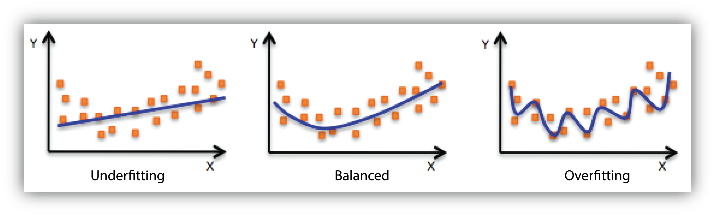
\includegraphics[width=0.7\textwidth]{under-overfitting.png}
    \caption{Ejemplo ilustrativo de subajuste, buen ajuste y sobreajuste en un modelo supervisado. Adaptado de \cite{awsOverfitting}.}
    \label{fig:overfitting}
\end{figure}

Existen varias categorías principales de aprendizaje automático, diferenciadas por la forma en que el algoritmo recibe la información 
y el tipo de tarea a resolver:
\begin{itemize}
    \item \textbf{Aprendizaje supervisado}: El algoritmo recibe ejemplos de entrada y su correspondiente salida deseada (etiquetas). 
    El objetivo es aprender una función que mapee las entradas a las salidas correctas. Son tareas típicas la \textit{clasificación} 
    (p. ej., dado un conjunto de características de un paciente, predecir que enfermedad tiene: salida categórica) y la 
    \textit{regresión} (p. ej., dada las características de una casa predecir su precio). El rendimiento se evalúa comúnmente con funciones
    que relacionan la predicción del modelo con el valor real (p. ej. error cuadrático en regressión o entropía cruzada en clasificación).

    \item \textbf{Aprendizaje no supervisado}: El algoritmo recibe datos de entrada sin etiquetas, y debe descubrir estructura oculta en 
    ellos. Incluye tareas como la \textit{clustering} (agrupamiento de datos por similitud) o la \textit{reducción de dimensionalidad} 
    (encontrar representaciones más compactas de los datos). Un claro ejemplo de aprendizaje no supervisado consiste en la agrupación de
    correos en distintos tipos.
    
    \item \textbf{Aprendizaje por refuerzo}: El algoritmo (un \textit{agente}) aprende a través de la interacción con un entorno, 
    recibiendo recompensas o penalizaciones según sus acciones. El agente debe descubrir una política de acciones que maximice la 
    recompensa acumulada. Este paradigma es común en robótica y juegos, donde no se proporcionan ejemplos de solución directa sino una 
    señal de calidad de cada acción.
    
\end{itemize}

En el ámbito médico se utiliza comunmente el \textbf{aprendizaje supervidado}. El proceso típico de esta tarea consiste en entrenar
un modelo ajustando sus parámetros para minimizar una función de error o \textit{función de pérdida} (loss function) que mide el error 
de las predicciones del modelo sobre los datos de entrenamiento. El procedimiento de optimización más utilizado es el 
\textit{descenso de gradiente} y sus variantes, como el descenso de gradiente estocástico, que permite procesar los datos por lotes. 
En cada iteración, se calcula la gradiente del error respecto a los parámetros del modelo, y se ajustan los parámetros en la dirección 
opuesta a dicha gradiente para reducir el error. Este ciclo se repite múltiples veces (\textit{épocas}) 
hasta converger a un mínimo local del error.

La Figura~\ref{fig:gd_flow} muestra esquemáticamente el flujo de este proceso, donde la posicion inicial tiene el error máximo y en cada
iteración se va reduciendo el error (como una pelota que rueda por una pendiente). A continuación, el Algoritmo~\ref{alg:gd-train} detalla 
los pasos fundamentales que se siguen durante el entrenamiento de un modelo mediante esta técnica.

\begin{figure}[ht]
    \centering
    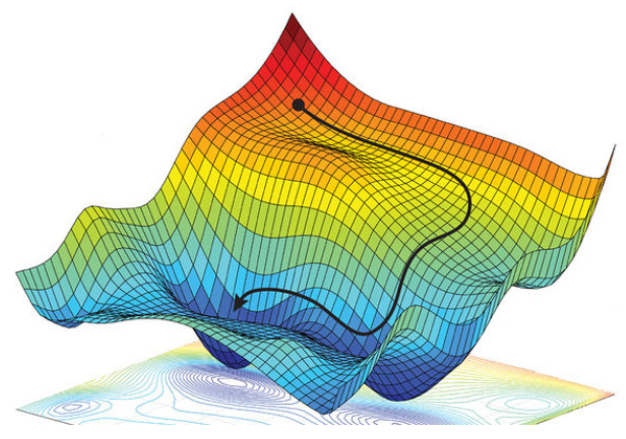
\includegraphics[width=0.8\textwidth]{descenso_gradiente.png}
    \caption{Flujo de entrenamiento de un modelo supervisado mediante descenso de gradiente. Adaptado de \cite{logongasBackprop}.}
    \label{fig:gd_flow}
\end{figure}

\begin{algorithmic}
    \label{alg:gd-train}
    \REQUIRE Conjunto de entrenamiento ${(x_i, y_i)}_{i=1}^N$, tasa de aprendizaje $\eta$ función de error $\mathcal{L}$
    \STATE Inicializar parámetros del modelo $\theta$ (p. ej. aleatoriamente)
    \FOR{numero de épocas}
        \FOR{cada $(x_i, y_i)$ en ${(x_i, y_i)}_{i=1}^N$}
            \STATE calcular predicción $\hat{y}_i = f_\theta(x_i)$
            \STATE calcular pérdida $L = \mathcal{L}(\hat{y}_i, y_i)$ \COMMENT{ej.: error cuadrático, entropía cruzada, etc.}
            \STATE calcular gradiente $g = \nabla_{\theta} L$
            \STATE actualizar parámetros: $\theta := \theta - \eta \cdot g$
        \ENDFOR
    \ENDFOR
\end{algorithmic}

Tras el entrenamiento, es fundamental evaluar el modelo con datos independientes (conjunto de \textit{prueba}) para estimar su capacidad de generalización. 
Además, suelen emplearse técnicas como \textit{validación cruzada} y conjuntos de \textit{validación} para ajustar hiperparámetros (parámetros del algoritmo 
que no se aprenden directamente, como la profundidad de un árbol de decisión o la tasa de aprendizaje $\eta$). Un buen enfoque de validación ayuda a prevenir 
el sobreajuste y a seleccionar modelos más robustos.

Existen algoritmos clásicos de ML como los \textit{árboles de decisión}, \textit{máquinas de vector soporte} (SVM), \textit{vecinos más cercanos} (k-NN), entre otros,
cada uno con sus supuestos y ámbitos de aplicación. Por ejemplo, las SVM buscan hiperplanos que separen clases maximizando el margen, mientras que los árboles de 
decisión realizan particiones recursivas del espacio de características para homogeneizar las etiquetas en los nodos hoja. La elección del algoritmo adecuado depende 
de la naturaleza de los datos y del problema a resolver, no existiendo un modelo único que sea óptimo para todas las tareas.

En resumen, el aprendizaje automático proporciona las bases para construir modelos que extraen conocimiento de los datos. Estos conceptos preliminares resultan 
imprescindibles para entender técnicas más avanzadas como las redes neuronales profundas y su aplicación en tareas de visión por computador y medicina, que se 
abordan en secciones posteriores.

\section{Redes Neuronales}\label{sec:nn} 

Las \textbf{redes neuronales artificiales} (RNA) constituyen una familia de modelos de aprendizaje automático inspirados vagamente en el cerebro humano. 
La unidad básica de una RNA es la \textit{neurona artificial}, un elemento que realiza una operación sencilla: calcula una combinación lineal de sus entradas y 
le aplica una función no lineal llamada \textit{función de activación}. Matemáticamente, si una neurona recibe como entradas $x_1, x_2, \dots, x_n$ con pesos 
sinápticos $w_1, w_2, \dots, w_n$ y tiene un sesgo $b$, produce una salida $y = \sigma(w_1 x_1 + w_2 x_2 + \cdots + w_n x_n + b)$, donde $\sigma(\cdot)$ podría ser, 
por ejemplo, una función sigmoide, tangente hiperbólica o ReLU (Unidad Lineal Rectificada). Las primeras RNA, como el \textit{Perceptrón} de Rosenblatt,  tenían una 
sola capa de neuronas (una capa de entrada proyectada directamente a una capa de salida) y podían aprender a clasificar datos que fueran linealmente separables. 
Sin embargo, se demostró que una sola neurona (o capa lineal) tiene limitaciones significativas en su capacidad de representación.

La potencia de las redes neuronales radica en su capacidad para formar \textbf{arquitecturas multicapa}, también conocidas como \textit{redes neuronales de múltiples capas} 
o \textit{perceptrones multicapa} (MLP). Estas redes están organizadas en capas: una capa de entrada (los datos originales), una o varias capas \textit{ocultas} que 
realizan transformaciones intermedias mediante neuronas con sus pesos, y una capa de salida que produce la predicción final. Al agregar capas ocultas con funciones de 
activación no lineales, las redes adquieren la habilidad de aproximar relaciones no lineales arbitrariamente complejas entre la entrada y la salida. En la imagen
\ref{fig:neural_network} se observa un ejemplo de una red neuronal profunda, donde cada círculo representa una neurona y las líneas indican las conexiones entre ellas.

\begin{figure}[htbp]
    \centering
    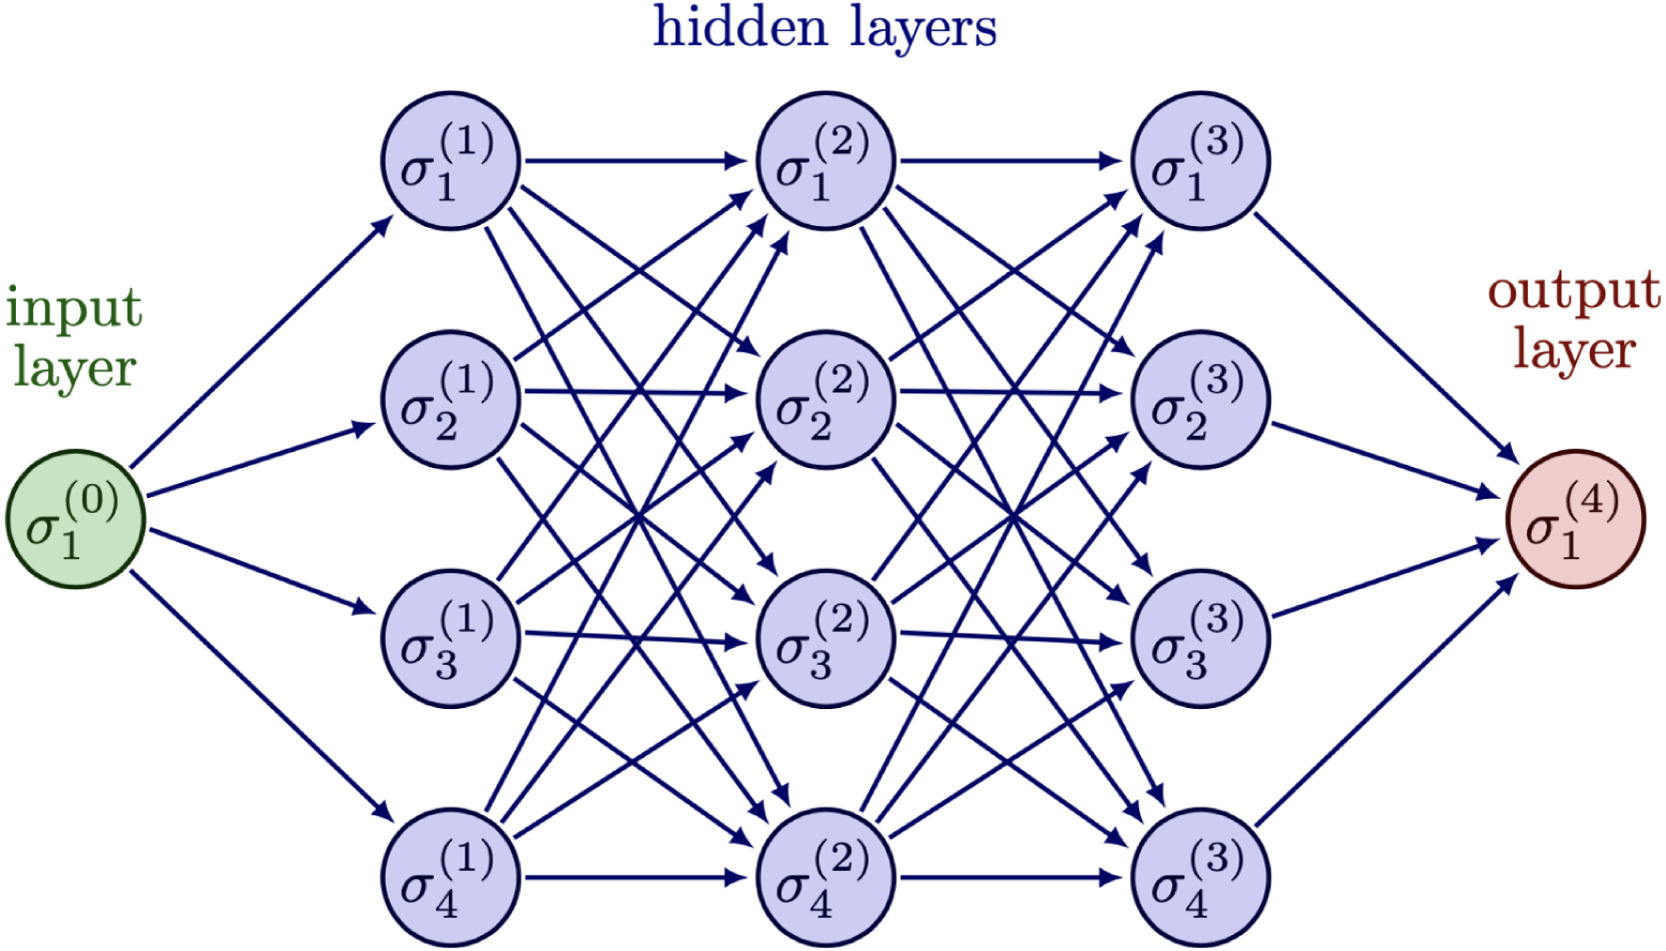
\includegraphics[width=0.5\textwidth]{neural_network.jpg}
    \caption{Ejemplo de una red neuronal profunda \cite{neural_network}}
    \label{fig:neural_network}
\end{figure}


El entrenamiento de una red neuronal multicapa se realiza típicamente mediante el algoritmo de \textit{retropropagación del error} (backpropagation) combinado con 
descenso de gradiente. En esencia, el procedimiento es: se calculan las salidas de la red para una entrada dada (\textit{fase forward}), se mide el error cometido 
comparando con la salida deseada mediante una función de coste (por ejemplo, la entropía cruzada para clasificación), y luego se propaga ese error hacia atrás a 
través de la red (\textit{fase backward}) calculando las derivadas parciales del error con respecto a cada peso utilizando la regla de la cadena. Estas derivadas 
indican cómo ajustar cada peso para reducir el error, y se aplican las actualizaciones de los pesos en consecuencia. Gracias a la retropropagación, las redes neuronales 
pueden entrenarse eficientemente incluso con muchas capas, ajustando millones de parámetros para adaptarse a complejos conjuntos de datos. Este avance fue crucial para 
el renacimiento de las redes neuronales en la década de 1980, tras un período de estancamiento parcial debido a las limitaciones de los perceptrones simples destacadas 
por Minsky y Papert en 1969 (quienes señalaron, por ejemplo, que un perceptrón no podía aprender la función XOR). El trabajo de Rumelhart, Hinton y Williams (1986) 
introdujo formalmente la retropropagación, mostrando que las redes de múltiples capas podían aprender características jerárquicas y superar esas limitaciones previas.

A medida que se dispuso de más datos y mayor potencia de cómputo, especialmente con la llegada de unidades de procesamiento gráfico (GPU) que aceleraron el cálculo 
matricial masivo, las redes neuronales crecieron en profundidad y capacidad. Surge así el campo del \textbf{aprendizaje profundo} (\textit{deep learning}), que no es 
más que el uso de redes neuronales con muchas capas (a veces decenas o incluso cientos) entrenadas sobre grandes volúmenes de datos. Un hito simbólico fue la competición 
ImageNet de 2012, en la cual una red convolucional profunda llamada \textit{AlexNet} obtuvo un rendimiento muy superior al de los métodos tradicionales en la tarea de 
clasificación de imágenes a gran escala. AlexNet, desarrollada por Krizhevsky et al. (2012), tenía 8 capas entrenables y introdujo técnicas como capas de \textit{dropout} 
para regularización y entrenamiento en GPU, marcando el inicio de una nueva era en visión por computador impulsada por redes neuronales profundas. Desde entonces, 
arquitecturas aún más profundas y sofisticadas han emergido, como \textit{VGGNet} (2014, 16-19 capas), \textit{Inception/GoogLeNet} (2015, con módulos de convolución 
en paralelo) y \textit{ResNet} (2016, más de 50 capas). En particular, las \textbf{redes residuales} (ResNets) de He et al. (2016) introdujeron conexiones de atajo 
(skip connections) que mitigaron el problema de la degradación del gradiente en redes muy profundas, permitiendo entrenar exitosamente redes de incluso 152 capas con 
mejoras significativas en la precisión de tareas de visión.

Una clase especial y sumamente importante de RNA para datos con estructura espacial o temporal son las \textbf{redes neuronales convolucionales} 
(CNN, por sus siglas en inglés). Las CNN fueron concebidas originalmente para procesar imágenes, inspiradas en la organización del córtex visual animal. 
En una CNN, en lugar de conectar todas las neuronas de una capa a todas las de la siguiente (como en un MLP denso tradicional), se emplean \textit{capas convolucionales} 
donde cada neurona está conectada solo a una región local de la capa anterior (campo receptivo) y todos los neuronas de una capa comparten conjuntos de pesos (filtros)
que se \textit{desplazan} sobre la entrada. Esta estructura explota las propiedades de \textit{estacionaridad} de las imágenes (patrones locales similares pueden 
aparecer en cualquier ubicación) y reduce drásticamente el número de parámetros al introducir \textit{pesos compartidos}. Además, se intercalan típicamente 
\textit{capas de pooling} (submuestreo), que reducen la resolución espacial agrupando activaciones cercanas (por ejemplo, tomando el máximo de cada bloque $2\times2$ 
de neuronas), confiriendo invarianza a traslaciones pequeñas y reduciendo la dimensionalidad progresivamente. Una arquitectura CNN típica para clasificación de 
imágenes consiste en varias capas convolucionales+pooling en cascada, que extraen características cada vez más abstractas de la imagen (bordes, texturas, partes, objetos), 
seguidas de una o más capas totalmente conectadas que actúan como clasificador final sobre esas características extraídas. La Figura \ref{fig:cnn_arch} muestra 
esquemáticamente un ejemplo de arquitectura CNN simple, con sus etapas de convolución, pooling y capas densas finales.

\begin{figure}[ht] \centering 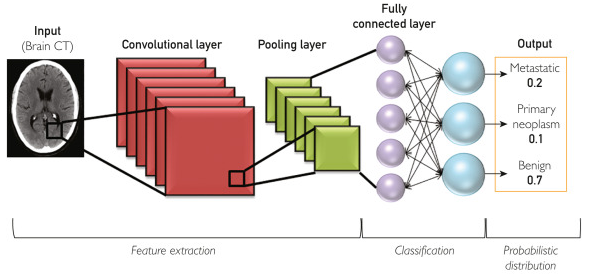
\includegraphics[width=0.8\textwidth]{cnn.png} 
    \caption{Ejemplo de arquitectura de una red neuronal convolucional para clasificación de imágenes. Se observan capas convolucionales (conv) que aplican 
    filtros aprendibles sobre la imagen de entrada, seguidas de capas de pooling que reducen la resolución. Al final, capas totalmente conectadas (FC) procesan 
    las características extraídas para producir la clasificación en alguna de las categorías.} 
    \label{fig:cnn_arch} 
\end{figure}

Las CNN han demostrado ser extremadamente efectivas en visión por computador, logrando reconocer objetos en fotos con gran precisión, segmentar imágenes píxel a píxel, 
detectar rostros, entre muchas otras aplicaciones. En el ámbito de imágenes médicas, han superado enfoques tradicionales al detectar patrones sutiles en radiografías, 
resonancias o microscopías que serían difíciles de modelar manualmente. No obstante, entrenar redes profundas con éxito requiere una gran cantidad de datos
clasificadas de manera manual, siendo de mayor dificultad en el ámbito médico donde la anotación de imágenes es costosa y requiere experiencia especializada.
Cuando el conjunto de datos disponible es limitado, es frecuente recurrir a \textit{aprendizaje por transferencia}, utilizando redes pre-entrenadas en un dominio 
amplio (p. ej., ImageNet) y refinándolas (fine-tuning) sobre la tarea específica, aprovechando características visuales genéricas aprendidas previamente.

Otro aspecto relevante es la \textit{interpretabilidad} de las predicciones de las redes neuronales. Las RNA profundas han sido criticadas como “cajas negras” 
difíciles de entender; sin embargo, se han desarrollado técnicas para visualizar y explicar qué han aprendido. Por ejemplo, en imágenes, métodos como \textit{Grad-CAM} 
(Gradiente-Weighted Class Activation Mapping) permiten resaltar las regiones de la imagen que más contribuyen a una determinada predicción de la red, proporcionando 
pistas sobre qué está “mirando” la CNN al tomar su decisión, pudiendo determinar si la red se basa en características relevantes o si ha aprendido patrones no generalizables
(p. ej. clasificando imagenes por el fondo en lugar del objeto de interés). 

En suma, las redes neuronales (especialmente las convolucionales profundas) constituyen la columna vertebral de muchos sistemas modernos de inteligencia artificial, 
logrando avances sin precedentes en reconocimiento de patrones. En la siguiente sección se explorará cómo estas técnicas de ML y redes neuronales se aplican en el ámbito de la visión por 
computador biomédica, con énfasis en el caso MedMNIST y la clasificación de artrosis en rodillas.

\section{ML aplicado a VC y tareas biomédicas: caso MedMNIST}\label{sec:ml-medical} 
La integración de técnicas de aprendizaje profundo y visión por computadora ha revolucionado el análisis de imágenes biomédicas en 
la última década. Tradicionalmente, la interpretación de imágenes médicas como radiografías, resonancias magnéticas y microscopías 
dependía exclusivamente de la habilidad humana. Sin embargo, en la actualidad, los algoritmos de \textit{deep learning} han igualado 
e incluso superado el desempeño de especialistas en diversas tareas diagnósticas.

Un ejemplo destacado es la empresa Quibim, fundada por el exalumno de la UPV, Ángel Alberich-Bayarri. Quibim ha desarrollado modelos 
basados en inteligencia artificial para la detección del cáncer de próstata en resonancias magnéticas. Su herramienta, QP-Prostate®, 
utiliza algoritmos avanzados para identificar y clasificar lesiones sospechosas en la glándula prostática, mejorando la precisión 
diagnóstica y facilitando la planificación de biopsias dirigidas.

Además, se han entrenado redes neuronales convolucionales para detectar retinopatía diabética en fotografías de retina, cáncer de 
piel en imágenes dermatoscópicas y neumonía en radiografías de tórax, alcanzando niveles de sensibilidad y especificidad 
comparables a los de médicos especialistas. Un metaanálisis realizado por Liu et al. (2019) concluyó que los clasificadores 
basados en aprendizaje profundo presentan, en promedio, un desempeño similar al de profesionales de la salud en la detección de 
enfermedades a partir de imágenes médicas, resaltando el potencial de estas técnicas para apoyar la labor clínica.

En el caso particular de la \textbf{artrosis de rodilla} (u osteoartritis), la radiografía es la técnica más utilizada para evaluar 
la gravedad de la enfermedad. Los radiólogos emplean un criterio estandarizado, la \textit{escala Kellgren-Lawrence (KL)}, que asigna 
un grado de 0 a 4 a la rodilla en función de signos radiográficos de degeneración (osteofitos, estrechamiento del espacio articular, 
esclerosis, deformidad). Sin embargo, la lectura de estas radiografías puede ser subjetiva y presentar variabilidad entre observadores.
Por ello, existe un gran interés en desarrollar sistemas automáticos que clasifiquen el grado KL a partir de la imagen de rayos X de 
la rodilla de forma consistente y reproducible. 

Dado el amplio espectro de modalidades y problemas en imágenes médicas, han surgido iniciativas para facilitar la investigación y 
comparación de algoritmos en múltiples tareas. Un ejemplo es la \textbf{Osteoarthritis Initiative (OAI)}, que ha desarrollado un conjunto 
de datos de radiografías de rodilla con anotaciones de grado Kellgren-Lawrence (KL) el cual se desarrollará mas adelante. 
Otro caso notable es \textbf{MedMNIST}, una colección de conjuntos de datos biomédicos de pequeño tamaño inspirada 
en el famoso MNIST (conjunto de datos de dígitos escritos a mano) pero orientada a imágenes médicas. En su versión más reciente, 
\textit{MedMNIST v2}, recopila 12 conjuntos de datos 2D (imágenes estáticas de 28$\times$28 píxeles) y 6 conjuntos 3D (volúmenes de 
28$\times$28$\times$28 vóxeles), abarcando diversas modalidades y tareas de clasificación biomédica. Por ejemplo, incluye láminas 
histológicas coloreadas (\textit{PathMNIST}, 9 clases de tejidos patológicos), imágenes dermatoscópicas de lunares (\textit{DermaMNIST}, 
clasificación de lesiones cutáneas) y radiografías de tórax (\textit{ChestMNIST}, etiquetas multilabel de hallazgos torácicos), 
hasta estudios de retina OCT (\textit{OCTMNIST}, detección de patologías retinales), entre otros. Cada subconjunto viene preprocesado 
y separado en particiones de entrenamiento, validación y prueba estandarizadas, lo que facilita la aplicación directa de algoritmos 
y la comparación justa entre ellos.

MedMNIST  fue diseñado con varios objetivos clave en mente:
\begin{itemize}
    \item \textbf{Diversidad}: Cubre múltiples modalidades de imagen (radiografías, tomografías, resonancias, ecografías, 
    imágenes microscopias, etc.), distintos tamaños de datos (desde $\sim$100 hasta $>$100,000 imágenes) y tareas de 
    clasificación variadas (binaria, multiclase, multietiqueta e incluso regresión ordinal). Esto permite evaluar la generalización 
    de los algoritmos de aprendizaje automático en distintos escenarios con un solo recurso unificado.
    
    \item \textbf{Estandarización}: Todos los conjuntos están uniformizados a la misma resolución (imágenes pequeñas de $28\times28$ 
    pixeles para 2D, o cubos de $28^3$ para 3D) con formato de datos consistente. Asimismo, se proveen divisiones oficiales en 
    entrenamiento/validación/test para cada dataset. Gracias a esto, los investigadores pueden centrarse en diseñar y probar 
    modelos de \textit{machine learning} sin preocuparse por el preprocesamiento de datos o posibles sesgos en la separación 
    de conjuntos, y los resultados son comparables entre diferentes estudios de forma más directa.
    
    \item \textbf{Ligereza y accesibilidad}:  El reducido tamaño de las imágenes hace que ejecutar experimentos sea computacionalmente 
    liviano, incluso sin hardware especializado. Además, la colección es de libre acceso con licencia abierta (CC BY) y cuenta con una 
    API unificada (disponible vía \texttt{pip install medmnist}) para cargar los datos fácilmente en diversos lenguajes. 
    Esto democratiza la experimentación en análisis de imágenes médicas, permitiendo a estudiantes y grupos con recursos limitados 
    explorar algoritmos de clasificación sobre datos reales de medicina.

    \item \textbf{Benchmark}: MedMNIST sirve tanto para introducir a nuevos usuarios en el campo de la visión médica, al 
    proporcionar casos ya preparados sobre los cuales practicar, como para benchmarking de algoritmos de AutoML y redes 
    neuronales en múltiples tareas livianas. Al enfocarse en imágenes pequeñas, enfatiza más el aspecto algorítmico 
    (diseño del modelo, estrategias de aprendizaje) que el meramente computacional. De hecho, trabajos asociados han 
    evaluado métodos clásicos de deep learning (ResNet, DenseNet, etc.) y herramientas AutoML sobre MedMNIST, generando 
    un punto de referencia inicial de desempeños.
\end{itemize}

En resumen, iniciativas como MedMNIST complementan a los grandes desafíos clínicos (ej. clasificar artrosis en radiografías 
completas) ofreciendo un “laboratorio” controlado para probar métodos de aprendizaje automático en imágenes biomédicas. 
El presente proyecto de TFG se enmarca precisamente en este contexto: la aplicación del aprendizaje automatico 
a la clasificación de artrosis de rodilla, un problema relevante en el campo de la salud musculoesquelética. 
Aprovechando conjuntos de datos como el de OAI \cite{chen2018knee} (con imágenes reales de pacientes) y los avances reportados 
en la literatura, se buscará entrenar un modelo capaz de predecir el estado de la articulación a partir de la radiografía, evaluando su desempeño 
y utilizando técncias de interpretación como \textit{Grad-CAM}. De este modo, se pretende contribuir tanto a la validación de las 
técnicas de aprendizaje profundo en una tarea biomédica específica como a la comprensión de sus alcances y limitaciones en 
un entorno clínico real.


%%%%%%%%%%%%%%%%%%%%%%%%%%%%%%%%%%%%%%%%%%%%%%%%%%%%%%%%%%%%%%%%%%%%%%%%%%%%%%%
%                              CAPÍTULO 3                                     %
%                     DESCRIPCIÓN DEL CORPUS DEL DATASET OAI                 %
%%%%%%%%%%%%%%%%%%%%%%%%%%%%%%%%%%%%%%%%%%%%%%%%%%%%%%%%%%%%%%%%%%%%%%%%%%%%%%%


\chapter{Corpus del Dataset OAI y tareas comunes}
\label{chap:corpus}

\section{Introducción al dataset OAI}

El estudio exhaustivo de la artrosis de rodilla (OA, por sus siglas en inglés \textit{Osteoarthritis}), una de las principales causas de dolor y discapacidad a nivel mundial, 
requiere imperativamente conjuntos de datos robustos, detallados y representativos. Estos datasets son cruciales no solo para investigar los complejos mecanismos subyacentes 
a la iniciación y progresión de la enfermedad, sino también para desarrollar y validar rigurosamente nuevas herramientas diagnósticas, pronósticas y terapéuticas. En este 
panorama, la \textit{Osteoarthritis Initiative (OAI)} \cite{niamsOAI} se destaca como uno de los recursos de investigación públicos más influyentes y extensamente utilizados 
por la comunidad científica internacional dedicada al estudio de la OA de rodilla. Establecida gracias a una colaboración público-privada liderada por los Institutos Nacionales 
de Salud de EE.UU. (NIH), la OAI fue lanzada oficialmente en 2004 como un estudio observacional, multicéntrico y longitudinal. Su objetivo primordial y ambicioso ha sido 
identificar y validar biomarcadores, que estén asociados de manera fiable con el desarrollo (incidencia) y el empeoramiento (progresión) de la OA de rodilla sintomática. 
Los datos generados por la OAI han impulsado numerosos avances en la comprensión de la enfermedad.

El diseño del estudio implicó el reclutamiento de una cohorte considerable de 4.796 participantes, con edades comprendidas entre los 45 y 79 años en el momento de la inclusión, 
distribuidos en cuatro centros clínicos de Estados Unidos (Universidad de Pittsburgh, Ohio State University, Universidad de Maryland y Memorial Hospital de Rhode Island). 
Estratégicamente, esta cohorte se diseñó para incluir tanto a individuos que ya presentaban OA de rodilla sintomática como a un grupo significativo de 
personas consideradas en alto riesgo de desarrollar la enfermedad (por factores como edad, sobrepeso, historial familiar o lesiones previas), pero sin diagnóstico confirmado 
al inicio. Esta composición heterogénea es particularmente valiosa porque permite investigar tanto los factores asociados a la aparición de la OA en individuos previamente 
sanos o en riesgo, como los determinantes de su progresión estructural y sintomática en aquellos ya afectados. Durante un periodo de seguimiento que se extendió por más de 
una década, se realizó una recopilación sistemática y estandarizada de una vasta cantidad de información en visitas periódicas (generalmente anuales, tras una evaluación basal 
exhaustiva). Estos datos incluyen detallados cuestionarios sobre síntomas (dolor, rigidez, función física - p.ej., usando escalas como WOMAC), exámenes físicos completos, 
mediciones de rendimiento físico, un extenso panel de análisis de biospecímenes (sangre, orina para biomarcadores solubles y genéticos), y, de forma central para muchos 
análisis, un protocolo riguroso de adquisición de imágenes médicas. Este protocolo incluye principalmente radiografías simples de ambas rodillas y resonancias magnéticas (RM) 
de alta resolución, obtenidas con secuencias específicas para evaluar el cartílago, meniscos, hueso subcondral y otras estructuras articulares.

Dentro del arsenal de datos de imagen recopilados por la OAI, las radiografías simples (rayos X) de rodilla continúan siendo un componente fundamental. Específicamente, 
las proyecciones posteroanteriores (PA) con la rodilla en flexión fija (\textit{fixed-flexion view}) se consideran el estándar de oro radiográfico para la evaluación clínica 
rutinaria y la clasificación de la severidad estructural de la OA. La popularidad de la radiografía se debe a su amplia disponibilidad, bajo 
coste relativo y su capacidad para visualizar características clave de la OA. La severidad radiográfica objetivada en estas imágenes se gradúa convencionalmente mediante la 
escala \textbf{Kellgren-Lawrence (KL)}, un sistema de clasificación semicuantitativo y ordinal propuesto originalmente en 1957. Esta escala 
evalúa globalmente la presencia y magnitud de varios signos radiográficos característicos de la OA, principalmente la formación de osteofitos (crecimientos óseos marginales) 
y el pinzamiento o estrechamiento del espacio articular (JSN, \textit{Joint Space Narrowing}), además de considerar la esclerosis subcondral y las deformidades óseas en los 
grados más avanzados. La escala KL distingue cinco grados de severidad, desde el grado 0 (ausencia de signos de OA) hasta el grado 4 (OA severa):

\begin{itemize}
    \item \textbf{Grado 0:} Normal. Sin características radiográficas de OA.
    \item \textbf{Grado 1:} Dudoso. Pinzamiento mínimo del espacio articular o posible formación de osteofitos marginales.
    \item \textbf{Grado 2:} Leve. Presencia definida de osteofitos y posible pinzamiento del espacio articular.
    \item \textbf{Grado 3:} Moderado. Osteofitos moderados múltiples, pinzamiento definido del espacio articular y posible esclerosis ósea leve.
    \item \textbf{Grado 4:} Severo. Grandes osteofitos, pinzamiento importante del espacio articular, esclerosis ósea marcada y deformidad ósea definida.
\end{itemize}

La Figura \ref{fig:knee-examples} muestra ejemplos visuales de radiografías correspondientes a cada uno de los grados KL. A pesar de su amplio uso, la escala KL presenta 
limitaciones conocidas, como su subjetividad y variabilidad interobservador, lo que motiva la búsqueda de métodos automáticos y objetivos para la evaluación de la OA 
\cite{chen2019fully}.

\begin{figure}[htbp]
    \centering
    \begin{subfigure}[b]{0.19\textwidth}
        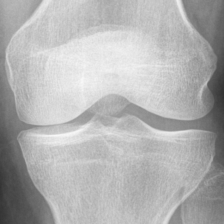
\includegraphics[width=\textwidth]{knee_0.png}
        \caption{KL 0}
        \label{fig:knee0}
    \end{subfigure}
    \hfill
    \begin{subfigure}[b]{0.19\textwidth}
        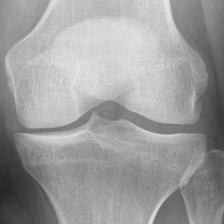
\includegraphics[width=\textwidth]{knee_1.png}
        \caption{KL 1}
        \label{fig:knee1}
    \end{subfigure}
    \hfill
    \begin{subfigure}[b]{0.19\textwidth}
        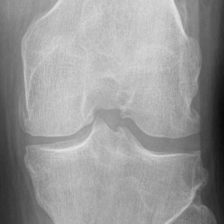
\includegraphics[width=\textwidth]{knee_2.png}
        \caption{KL 2}
        \label{fig:knee2}
    \end{subfigure}
    \hfill
    \begin{subfigure}[b]{0.19\textwidth}
        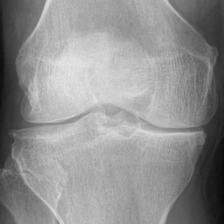
\includegraphics[width=\textwidth]{knee_3.png}
        \caption{KL 3}
        \label{fig:knee3}
    \end{subfigure}
    \hfill
    \begin{subfigure}[b]{0.19\textwidth}
        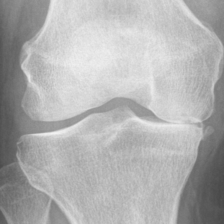
\includegraphics[width=\textwidth]{knee_4.png}
        \caption{KL 4}
        \label{fig:knee4}
    \end{subfigure}
    \caption{Ejemplos de radiografías de rodilla clasificadas según la escala Kellgren \& Lawrence (KL)}
    \label{fig:knee-examples}
\end{figure}

Este conjunto de datos constituye la base del presente Trabajo de Fin de Grado, ya que proporciona imágenes de rodilla etiquetadas 
con el grado de artrosis según la escala KL. Gracias a su fiabilidad y a su estructura previamente curada, permite el entrenamiento
de redes neuronales convolucionales de manera reproducible, facilitando la comparación con estudios previos y la validación de nuevas 
propuestas de clasificación automática en imágenes médicas.

% --- Características del Dataset (Versión Mendeley/Kaggle) ---
\section{Características del Dataset (Versión Mendeley/Kaggle)}
\label{sec:dataset_characteristics}

Si bien la base de datos completa de la OAI es extraordinariamente rica, su gran volumen y complejidad estructural pueden dificultar su uso directo para tareas específicas de 
aprendizaje automático, como el entrenamiento de modelos de clasificación de imágenes. Por esta razón, diversos investigadores han creado y distribuido públicamente 
versiones curadas y procesadas de subconjuntos de datos radiográficos del OAI. Estas versiones facilitan enormemente el acceso y la aplicación de técnicas de inteligencia 
artificial. Dos de las plataformas donde se encuentran frecuentemente estas versiones adaptadas son Mendeley Data, como el conjunto de datos publicado por Chen (2018) 
\cite{chen2018knee} pudiendose encontrar en Mendeley y Kaggle, dataset utilizado en numerosos trabajos.

El dataset publicado en Mendeley Data por Chen, estrechamente vinculado a su trabajo posterior sobre clasificación automática de grados KL mediante 
redes neuronales profundas \cite{chen2019fully}, es un ejemplo prominente y fue específicamente organizado para facilitar tareas de detección de la articulación y clasificación 
de la severidad. Las características generales de estas versiones procesadas, que constituyen la base de numerosos estudios posteriores (incluido el presente trabajo), suelen ser 
las siguientes:

\begin{itemize}
    \item \textbf{Imágenes:} El conjunto total incluye \textbf{9\,786 imágenes}, distribuidas en cuatro particiones diferenciadas: \textit{train} (5\,778), \textit{validation} (826), \textit{test} (1\,656) y \textit{auto\_test} (1\,526), como se muestra en la Tabla~\ref{tab:splits}.
    
    \begin{table}[h]
        \centering
        \caption{Distribución de imágenes por partición}
        \label{tab:splits}
        \begin{tabular}{lrr}
            \toprule
            \textbf{Partición} & \textbf{Número de imágenes} & \textbf{Porcentaje} \\
            \midrule
            Entrenamiento (Train) & 5\,778 & 59.04\,\% \\
            Validación (Validation) & 826 & 8.44\,\% \\
            Prueba (Test) & 1\,656 & 16.92\,\% \\
            Autoevaluación (AutoTest) & 1\,526 & 15.59\,\% \\
            \bottomrule
        \end{tabular}
    \end{table}

    \begin{figure}[ht]
        \centering
        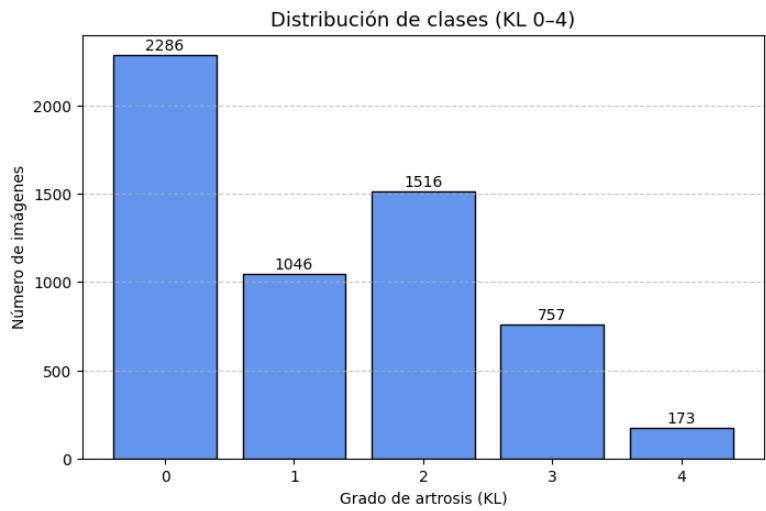
\includegraphics[width=0.6\textwidth]{class_distribution_train.png}
        \caption{Distribución de clases (KL 0 a KL 4) en el conjunto de entrenamiento del dataset OAI. Se observa un desbalance significativo hacia los grados más leves.}
        \label{fig:class_barplot}
    \end{figure}

    \item \textbf{Etiquetas:} Cada imagen está etiquetada con un grado KL (de 0 a 4), siguiendo el criterio de radiólogos expertos de la OAI. Esta información es clave 
    para entrenar modelos supervisados de clasificación.

    \item \textbf{Resolución y preprocesamiento:} En la versión de Mendeley, las imágenes se encuentran disponibles en dos resoluciones estándar: \textbf{224x224} y 
    \textbf{299x299} píxeles, facilitando el uso de arquitecturas preentrenadas como ResNet o EfficientNet. En la versión de Kaggle solo están disponibles en 224x224
    píxeles, lo que la hace más directa para su uso en modelos CNN comunes.

    \item \textbf{Distribución de clases:} La Tabla~\ref{tab:class_distribution} muestra la distribución de clases en el conjunto de entrenamiento. Se observa un claro 
    desbalance hacia las clases más leves de artrosis, lo que debe considerarse en el diseño de los modelos de clasificación.

    \begin{table}[h]
        \centering
        \caption{Distribución de clases en el conjunto de entrenamiento}
        \label{tab:class_distribution}
        \begin{tabular}{lrrrr}
            \toprule
            \textbf{Clase KL} & \textbf{Índice} & \textbf{Imágenes} & \textbf{Porcentaje} \\
            \midrule
            0 (Sin artrosis) & 0 & 2\,286 & 39.56\,\% \\
            1 (Ligera) & 1 & 1\,046 & 18.10\,\% \\
            2 (Leve) & 2 & 1\,516 & 26.24\,\% \\
            3 (Moderada) & 3 & 757 & 13.10\,\% \\
            4 (Severa) & 4 & 173 & 2.99\,\% \\
            \bottomrule
        \end{tabular}
    \end{table}

    Como se observa, el conjunto de entrenamiento presenta un notable desbalance de clases, con predominancia de imágenes etiquetadas con 
    grado 0 (sin artrosis) y grado 2 (leve), y una clara escasez de imágenes con grado 4 (severa). Este desbalance puede inducir a que el modelo 
    favorezca las clases más frecuentes durante el entrenamiento, afectando negativamente su capacidad para detectar los casos más críticos. 

    \item \textbf{Divisiones (Splits):} La existencia de splits predefinidos facilita la reproducibilidad de experimentos y la comparación entre distintos enfoques. 
    Considerando únicamente los subconjuntos \textit{train}, \textit{validation} y \textit{test} —que son los habitualmente utilizados para entrenar y evaluar modelos— 
    se mantiene una proporción aproximada de \textbf{70\,\% entrenamiento}, \textbf{10\,\% validación} y \textbf{20\,\% test}, ampliamente adoptada en la comunidad. 
    El conjunto \textit{auto\_test}, aunque no se utiliza en todos los trabajos, está disponible como recurso adicional que se utiliza en ocasiones para aumentar la cantidad de 
    imagenes en el entrenamiento.
\end{itemize}

\section{Taras comunes en el dataset OAI}
\label{sec:common_tasks}

El conjunto de datos de la *Osteoarthritis Initiative* (OAI) ha sido ampliamente empleado en la literatura científica como base para el desarrollo de modelos de aprendizaje
profundo orientados al diagnóstico automatizado de la artrosis de rodilla. Gracias a su riqueza clínica y su volumen de imágenes radiográficas etiquetadas según la escala de
Kellgren-Lawrence (KL), este dataset se ha convertido en una referencia para la validación de nuevas arquitecturas y metodologías dentro del ámbito de la inteligencia 
artificial aplicada a la medicina.

A lo largo del tiempo, diferentes líneas de investigación han coincidido en una serie de tareas recurrentes que abordan distintos enfoques sobre la severidad de la artrosis. 
Estas tareas pueden clasificarse, principalmente, en función de tres criterios:

\begin{itemize}
    \item El tipo de clasificación: binaria (presencia o ausencia de artrosis) o multiclase (grados de KL de 0 a 4).
    \item La metodología de entrenamiento: desde cero (*from scratch*) o mediante *transfer learning* con redes preentrenadas.
    \item La formulación del problema: como clasificación ordinaria o regresión ordinal.
\end{itemize}

Cabe destacar que estas tareas no son excluyentes, y muchas publicaciones recientes exploran combinaciones de estos enfoques. Además, se ha popularizado el uso de técnicas complementarias 
como el ensamblado de modelos (ensembling), el ajuste fino de pesos (fine-tuning) o el uso de funciones de pérdida adaptadas a la naturaleza ordinal del problema.

En el contexto de este Trabajo de Fin de Grado, el foco se centrará exclusivamente en la tarea de clasificación del grado de artrosis, descartando explícitamente la tarea de detección automática de 
la articulación de la rodilla. Se parte de imágenes radiográficas previamente recortadas como se encuentran en los datasets disponibles en Mendeley y Kaggle, donde la articulación ya ha sido
detectada y centrada, pudiendo replicar los experimentos de otros autores y comparar los resultados obtenidos de una manera más directa. 

A modo de ejemplo representativo de las tareas descritas, se presentan a continuación varios estudios recientes que han abordado el problema de clasificación de la artrosis de 
rodilla utilizando el dataset OAI, cada uno desde una perspectiva metodológica distinta. Estos trabajos ilustran bien la diversidad de aproximaciones y motivaciones que existen 
en la literatura científica actual, y permiten contextualizar el enfoque adoptado en este Trabajo de Fin de Grado.

\textbf{Chen et al. (2019)} \cite{chen2019fully} desarrollan un sistema completamente automatizado para la clasificación de la severidad de la 
artrosis de rodilla, combinando detección de la articulación con YOLOv2 y posterior clasificación mediante redes neuronales profundas. 
En el contexto de este TFG, el interés se centra en la segunda fase del pipeline: la predicción del grado de artrosis según la escala de 
Kellgren-Lawrence (KL). Los autores emplean arquitecturas CNN preentrenadas como VGG, ResNet, InceptionV3 y DenseNet, afinadas con una función de 
pérdida personalizada denominada adjustable ordinal loss, diseñada para penalizar más severamente los errores a mayor distancia ordinal. 
Los resultados muestran que esta función mejora el rendimiento frente a la entropía cruzada tradicional, alcanzando una precisión del 70.4\% con 
VGG-19 como mejor modelo. Esta propuesta es destacable por introducir de manera explícita la naturaleza ordinal de las etiquetas KL en el proceso 
de entrenamiento, aspecto esencial para tareas clínicas con niveles de severidad escalonados.

\textbf{Srikijkasemwat et al. (2024)} \cite{kneexnet2024} presentan KneeXNet, un sistema basado en ensamblado de modelos para la clasificación 
automática del grado de artrosis a partir de radiografías del dataset OAI. Evalúan diez modelos preentrenados en ImageNet —incluyendo ResNet, 
VGG, DenseNet, EfficientNet y GoogLeNet— y aplican dos estrategias de fusión: votación mayoritaria y una red neuronal superficial. Además, 
integran técnicas como muestreo ponderado para lidiar con el desequilibrio de clases y Smooth-GradCAM++ para mejorar la interpretabilidad. 
El modelo ensamblado mediante red superficial alcanza una precisión del 72\%, superando individualmente a cada arquitectura evaluada.
Este trabajo subraya la utilidad del ensamblado y de la explicabilidad en escenarios clínicos, aportando un marco sólido con el que se pueden 
comparar propuestas futuras.

\textbf{Nabil et al. (2024)} \cite{nabil2024automatic} optan por una estrategia simplificada que agrupa las clases KL 0, 1 y 2 bajo la categoría 
“sano”, lo cual responde a la dificultad recurrente en la clasificación precisa del grado KL1. Comparan tres arquitecturas profundas 
—EfficientNetB7, DenseNet169 e InceptionResNetV2— y reportan un rendimiento superior de EfficientNetB7, con una precisión del 93.90\%. 
Su propuesta destaca por una cuidadosa fase de preprocesamiento, uso extensivo de técnicas de aumento de datos y regularización, así 
como una formulación del problema como clasificación en tres niveles (sano, moderado, severo). Pese a su elevado coste computacional, 
EfficientNetB7 se presenta como una solución idónea para entornos clínicos donde la precisión diagnóstica es prioritaria.

\textbf{Fei et al. (2024)} \cite{fei2024diagnosing} plantean un cambio conceptual al abordar la clasificación de la artrosis como un problema 
de regresión continua, en lugar de una clasificación discreta. Utilizando redes neuronales convolucionales, sus modelos generan puntuaciones 
decimales entre 0 y 4 que reflejan con mayor precisión la progresión de la enfermedad. Evalúan cuatro arquitecturas —VGG16, ResNet34, 
DenseNet196 y EfficientNetV2 small— sobre 8260 imágenes del dataset OAI, siendo EfficientNetV2 la más destacada, con una precisión del 71\%, 
AUC de 0.83 y un error absoluto medio (MAE) de 0.42. Este enfoque permite un análisis más granular y continuo del estado articular, abriendo 
la puerta a aplicaciones como el seguimiento longitudinal, la predicción de progresión y el soporte a la decisión clínica.

Cabe destacar que, al igual que la función de pérdida adjustable ordinal loss utilizada por Chen et al. (2019), el uso de una pérdida de tipo 
error cuadrático medio en este estudio refleja la intención de penalizar proporcionalmente según la distancia ordinal entre la predicción y 
la etiqueta real. Aunque desde una perspectiva técnica se trata de una formulación regresiva en lugar de categórica, ambas propuestas comparten 
el objetivo de capturar la estructura ordinal inherente al sistema de gradación de Kellgren-Lawrence, superando así las limitaciones de la entropía 
cruzada convencional.

En la Tabla~\ref{tab:comparative_oai} se presenta una síntesis comparativa de los principales trabajos analizados que han utilizado el dataset OAI. 
Se resumen los modelos empleados, el tipo de tarea formulada, las métricas clave reportadas y observaciones destacadas de cada enfoque. Esta 
comparativa permite tener una visión global del panorama actual, así como identificar tendencias metodológicas relevantes para este TFG.

\begin{table}[h]
    \centering
    \caption{Comparativa de trabajos previos con el dataset OAI}
    \label{tab:comparative_oai}
    \begin{tabular}{lllll}
        \toprule
        \textbf{Estudio} & \textbf{Tarea} & \textbf{Precisión} & \textbf{Observaciones} \\
        \midrule
        Chen et al. (2019) & Clasificación ordinal & 70.4\% & Adjustable loss \\
        Srikijkasemwat et al. (2024) & Multiclase & 72\% & Interpretabilidad \\
        Nabil et al. (2024)  & Binaria (agrupada) & 93.9*\%  & Aumento de datos \\
        Fei et al. (2024)  & Regresión & 71\% & Output continuo \\
        \bottomrule
    \end{tabular}
\end{table}

El análisis de estos trabajos evidencia una creciente tendencia a incorporar la naturaleza ordinal del problema, así como a experimentar 
con formulaciones alternativas como la regresión o el uso de modelos ensamblados. Esta revisión proporciona una base sólida para el diseño 
experimental planteado en los capítulos siguientes, donde se compararán distintos enfoques de clasificación aplicados sobre el dataset OAI, 
considerando también la interpretación de resultados mediante técnicas como Grad-CAM.


%%%%%%%%%%%%%%%%%%%%%%%%%%%%%%%%%%%%%%%%%%%%%%%%%%%%%%%%%%%%%%%%%%%%%%%%%%%%%%%

\chapter{Capítulo 4 | Contribución 1: Experimentación y Análisis de Resultados}
\label{chap:experiments}

Experimentos hechos con el dataset de kaggle replicando papers

\chapter{Capítulo X | contribución 1: Experimentación y Análisis de Resultados}

\section{Introducción}
En este capítulo se presentan los experimentos realizados para evaluar el desempeño de diversas arquitecturas de redes neuronales en la detección de artrosis en rodillas. Con el objetivo de aportar evidencia empírica para la detección temprana de la enfermedad, se han probado variantes de modelos EfficientNet y ResNet utilizando dos estrategias de entrenamiento: el uso de pesos pre-entrenados (transfer learning) y el entrenamiento desde cero (\textit{from scratch}). Los experimentos se han llevado a cabo sobre el conjunto de datos Mendeley \cite{chen2018knee} y se han tomado como referencia las aportaciones teóricas y experimentales descritas en \cite{efficientnet_paper}. 

\section{Metodología Experimental}

\subsection{Configuración del Experimento}
Para todos los experimentos se siguió el siguiente protocolo:
\begin{itemize}
    \item \textbf{Preprocesamiento:} Se redimensionaron las imágenes a un tamaño uniforme (224x224), se aplicaron técnicas de histogram equalization y bilateral filtering y transformación de la imagen a RGB. Aparte de un aumentos de datos (flip horizontal y vertical) para mejorar la generalización del modelo.
    \item \textbf{Partición del Conjunto de Datos:} El dataset se dividió en subconjuntos de entrenamiento, validación y prueba, siguiendo los porcentajes previamente establecidos. 75\% para entrenamiento, 17\% para prueba y 8\% para validación.
    \item \textbf{Configuración de Entrenamiento:} Se usó la función de pérdida \textit{Categorical Cross-Entropy} y el optimizador Adam con una tasa de aprendizaje inicial de 0.001, aplicando un scheduler para la reducción de la tasa en caso de estancamiento. Se entrenó hasta 50 épocas, implementando técnicas de Early Stopping para evitar sobreajuste. También se aplicó regularización L2 con valores entre 0.001 y 0.0001 para prevenir el sobreajuste.
\end{itemize}

\subsection{Modelos Evaluados}
Se evaluaron las siguientes arquitecturas:
\begin{itemize}
    \item \textbf{EfficientNet:} De la familia se probaron los modelos B0, B4, B5 y B7
    \item \textbf{ResNet50:} Modelo representativo de la familia ResNet.
\end{itemize}

\subsection{Estrategias de Entrenamiento}
Se compararon dos enfoques:
\begin{enumerate}
    \item \textbf{Transfer Learning:} Utilizando pesos pre-entrenados en grandes bases de datos (por ejemplo, ImageNet) para adaptar el modelo a la tarea específica de clasificación de artrosis.
    \item \textbf{Entrenamiento Desde Cero (\textit{From Scratch}):} Inicializando los pesos de manera aleatoria y entrenando la red sin conocimiento previo.
\end{enumerate}

\section{Resultados Experimentales}

\subsection{Comparación de Arquitecturas y Estrategias}
Los experimentos demostraron que, en su mayoría, tanto los modelos EfficientNet como los ResNet alcanzaron precisiones cercanas al 70\%, excepto EfficientNetB5 que logró una precisión del 71\%. La Tabla \ref{tab:resultados_experimentos} resume los resultados obtenidos.
La precisión obtenida se escogió en base a la época de entrenamiento con menor pérdida. En algunos casos los modelos conseguian una mejor precisión con mayor perdida, pero no siendo significativa la mejora.
\begin{table}[htbp]
\centering
\begin{tabular}{lccc}
\toprule
\textbf{Modelo y Estrategia} & \textbf{Precisión (\%)} & \textbf{Val loss} & \textbf{Épocas necesarias} \\
\midrule
EfficientNetB0 (Pre-entrenado)  & 69.87\%    & 0.73 & 7 \\
EfficientNetB5 (Pre-entrenado)  & 72.82\%    & 0.81 & 2 \\
EfficientNetB7 (Pre-entrenado)  & 66.54\%    & 0.79 & 13 \\
EfficientNetB4 (Desde Cero)     & 59.36\%    & 0.96 & 49 \\
ResNet50 (Pre-entrenado)        & 66.66\%    & 0.78 & 4 \\
ResNet50 (Desde Cero)           & 65.89\%    & 0.84 & 28 \\

\bottomrule
\end{tabular}
\caption{Comparación de modelos y estrategias de entrenamiento}
\label{tab:resultados_experimentos}
\end{table}

\begin{figure}[htbp]
    \centering
    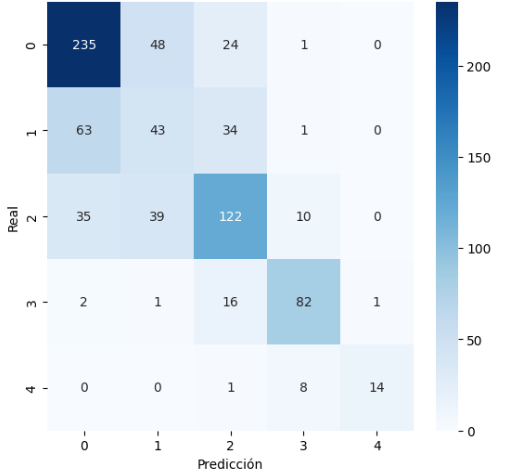
\includegraphics[width=0.6\textwidth]{EfficientNet_B7.png}
    \caption{Descripción de la imagen}
    \label{fig:matriz_confusion}
\end{figure}

\subsection{Impacto del Uso de Pesos Pre-entrenados}
Los experimentos evidenciaron que:
\begin{itemize}
    \item \textbf{Convergencia Rápida:} Los modelos con pesos pre-entrenados alcanzaron la convergencia en menos épocas, reduciendo significativamente el tiempo de entrenamiento.
    \item \textbf{Mayor Precisión:} Se observó un aumento en la precisión (hasta 71\% en el caso de EfficientNetB5) en comparación con el entrenamiento desde cero, donde los resultados se situaron en torno al 67-68\%.
    \item \textbf{Robustez del Modelo:} Los modelos pre-entrenados realizaban un overfitting mas pronunciado, pero la precisión obtenida era mayor que los modelos entrenados desde cero.
\end{itemize}

\subsection{Análisis Comparativo y Discusión}
La comparación entre los dos enfoques de entrenamiento resalta la importancia de la transferencia de aprendizaje en el dominio biomédico:
\begin{itemize}
    \item Aunque la mejora en precisión entre modelos pre-entrenados y entrenados desde cero es modesta (aproximadamente un 1-2\%), esta diferencia es crucial en aplicaciones clínicas, donde cada punto porcentual puede tener un impacto significativo en el diagnóstico.
    \item El entrenamiento desde cero presentó desventajas claras, tales como un mayor consumo de recursos computacionales y un tiempo de entrenamiento considerablemente más largo, lo cual puede ser prohibitivo en entornos con recursos limitados.
    \item EfficientNetB5 destacó frente a las demás arquitecturas, lo que sugiere que una mayor capacidad del modelo (a pesar de aumentar la complejidad) puede traducirse en mejoras en el desempeño, siempre y cuando se disponga de una estrategia de entrenamiento adecuada.
\end{itemize}

\section{Conclusiones del Capítulo}
Los experimentos realizados permiten concluir que:

\cleardoublepage


\chapter{Capítulo 2 de contribución}   % ~15 páginas
% Expón aquí tu segundo objetivo y resultados derivados

%%%%%%%%%%%%%%%%%%%%%%%%%%%%%%%%%%%%%%%%%%%%%%%%%%%%%%%%%%%%%%%%%%%%%%%%%%%%%%%
%                              CAPÍTULO 5                                     %
%                     TERCERA CONTRIBUCIÓN (OBJETIVO 3)                       %
%%%%%%%%%%%%%%%%%%%%%%%%%%%%%%%%%%%%%%%%%%%%%%%%%%%%%%%%%%%%%%%%%%%%%%%%%%%%%%%

\chapter{Capítulo 3 de contribución}   % ~15 páginas
% Expón aquí tu tercer objetivo y resultados derivados

%%%%%%%%%%%%%%%%%%%%%%%%%%%%%%%%%%%%%%%%%%%%%%%%%%%%%%%%%%%%%%%%%%%%%%%%%%%%%%%
%                              CAPÍTULO 6                                     %
%                                CONCLUSIONES                                 %
%%%%%%%%%%%%%%%%%%%%%%%%%%%%%%%%%%%%%%%%%%%%%%%%%%%%%%%%%%%%%%%%%%%%%%%%%%%%%%%

\chapter{Conclusiones}  % ~5 páginas

\section{Resumen del trabajo realizado} % 6.1
% Repasa y sintetiza las secciones principales

\section{Objetivos alcanzados}         % 6.2
% Verifica si se cumplieron los objetivos planteados

\section{Trabajo futuro}               % 6.3
% Explica las posibles extensiones o mejoras

%%%%%%%%%%%%%%%%%%%%%%%%%%%%%%%%%%%%%%%%%%%%%%%%%%%%%%%%%%%%%%%%%%%%%%%%%%%%%%%
%                              BIBLIOGRAFÍA                                   %
%%%%%%%%%%%%%%%%%%%%%%%%%%%%%%%%%%%%%%%%%%%%%%%%%%%%%%%%%%%%%%%%%%%%%%%%%%%%%%%

\printbibliography 
\cleardoublepage

%%%%%%%%%%%%%%%%%%%%%%%%%%%%%%%%%%%%%%%%%%%%%%%%%%%%%%%%%%%%%%%%%%%%%%%%%%%%%%%
%                           APÉNDICES (OPCIONALES)                            %
%%%%%%%%%%%%%%%%%%%%%%%%%%%%%%%%%%%%%%%%%%%%%%%%%%%%%%%%%%%%%%%%%%%%%%%%%%%%%%%

\APPENDIX

\chapter{Configuración del sistema}
% ...

\chapter{Otro apéndice}
% ...

\end{document}
